
\documentclass[a4paper,11pt]{book}
\usepackage[T1]{fontenc}
\usepackage[utf8]{inputenc}
\usepackage{lmodern}

\usepackage{hyperref}
\usepackage{graphicx}
\usepackage[portuguese]{babel}
\graphicspath{ {images/} }

\title{\Huge \textbf{Game of Life}  \huge Manual do utilizador e breve análise dos resultados}

\author{\textsc{Afonso Rufino e Dinis Rocha}}


\begin{document}

\frontmatter
\maketitle

\tableofcontents

\mainmatter

\chapter{Introdução}
\paragraph{}
O Game of Life é um autómato celular inventado pelo matemático britânico John Conway em 1970 e desde então, tornou-se bastante popular. É um jogo de zero jogadores, significando que a sua evolução é determinada pelo estado inicial, não requerendo mais nenhuma interação do utilizador. Dada a sua popularidade, conduziu-se um estudo exaustivo de padrões especiais, desde o tradicional “glider” a inteiros computadores Turing-completos.
\paragraph{} Toda a evolução que se verifica no Jogo decorre de 3 simples regras, que dão origem a uma nova configuração quando aplicadas à anterior. São elas:

\begin{itemize}
\item Qualquer célula viva com mais de três vizinhos morre.
\item Qualquer célula morta com três vizinhos vivos torna-se viva
\item Qualquer célula com 2 ou 3 vizinhos vivos continua no mesmo estado na configuração seguinte
\end{itemize}
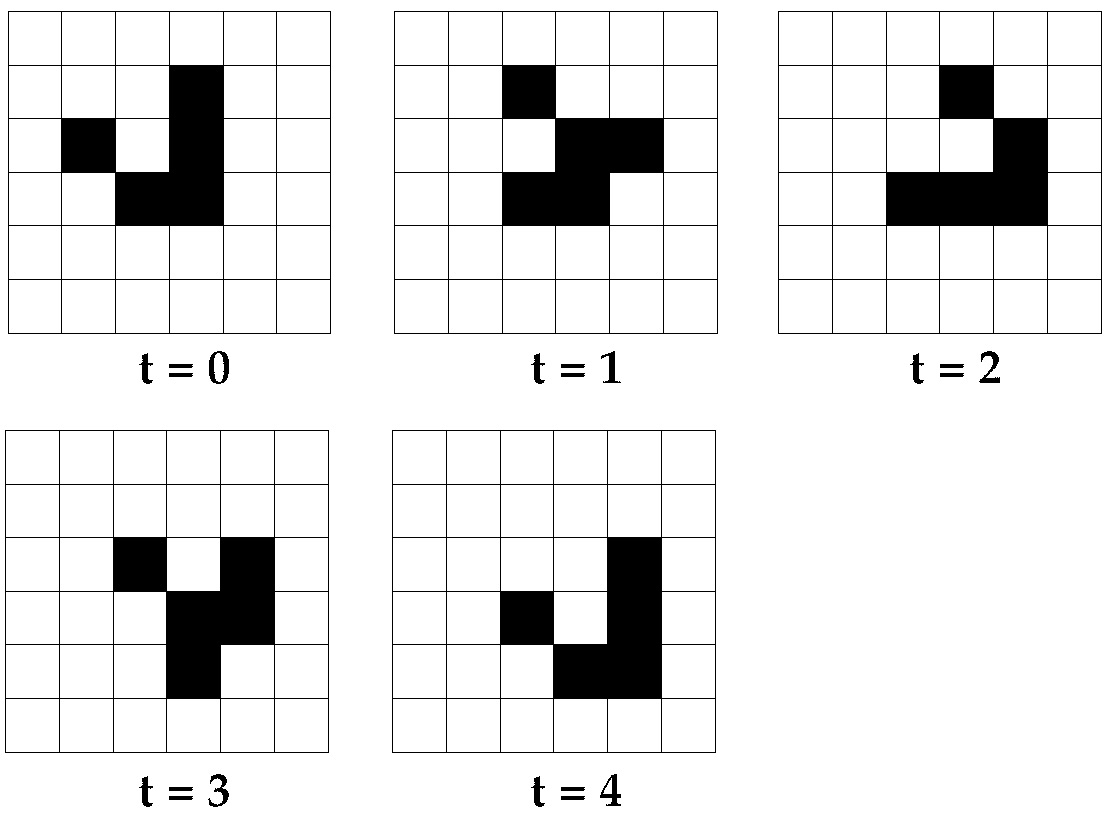
\includegraphics[scale = 0.2]{glider}

\paragraph{}Na nossa abordagem ao Jogo da Vida, começamos por definir estas regras. Posteriormente, quisemos explorar uma outra possibilidade: dada uma probabilidade de estas regras não serem seguidas (evento “quântico”), de que forma evolui o Jogo? A partir de uma configuração nula, é possível que surjam espontaneamente estruturas complexas?
\paragraph{}Com esta finalidade, desenvolvemos dois programas que partilham a lógica por trás da alteração das configurações.
\paragraph{Versão Gtk}Inclui uma interface gráfica, que permite observar a simulação, bem como gráficos que representam a evolução do sistema em função do tempo. Permite ainda gerar aleatoriamente, editar diretamente, guardar e importar configurações. 
\paragraph{Versão Dev } Sem interface gráfica, otimizada para calcular muitas iterações rapidamente, ao qual recorremos para fazer um estudo do surgimento de estruturas complexas em função da probabilidade. Encorajamos o utilizador a complementar a nossa breve investigação, utilizando e modificando esse mesmo programa.
\chapter {Manual do Utilizador}
\section{Controlo a partir do teclado}

\begin{tabular}{|r|l|}
  \hline
  + & "zoom in" no ecrã da simulação (aumenta o tamanho de cada célula) \\
  - & “zoom out” no ecrã da simulação (diminui o tamanho de cada célula) \\
  w & translação da simulação para cima no ecrã \\
  a  & translação da simulação para a esquerda no ecrã\\
  s & translação da simulação para baixo no ecrã\\
  d &  translação da simulação para a direita no ecrã \\
  r & repõe todas as configurações para as suas predefinições \\
  \hline
\end{tabular}

\section{Controlo a partir do Rato}
  \begin{itemize}
      \item Clicar com o botão esquerdo do rato para tornar uma célula viva;
      \item Clicar com o botão direito do rato para tornar uma célula morta;
  \end{itemize}

\section{Botões}
\begin{itemize}
    \item “Pause/play”: para ou continua a simulação;
    \item “Choose M” , “Choose N”,  “Choose Probability” e “Generate new config”: os spin buttons permitem escolher os parâmetros para uma nova configuração aleatória, que é gerada quando se clica no último dos botões;
    \item “Enable quantum mode” e “Quantum probability”: permitem, respetivamente, ativar e escolher a probabilidade do modo quântico;
    \item “Save configuration in file”: permite guardar o estado  atual do Jogo num ficheiro binário. Abre um “file chooser dialog” que permite ao utilizador escolher o nome e a localização do ficheiro.
    \item “Load configuration from file”: permite importar uma configuração de um ficheiro binário de configurações anteriormente criado pelo programa. AVISO: Não tentar abrir um ficheiro que não tenha sido gerado por um dos programas de Jogo da Vida, pois isso levará o programa a parar. Algumas configurações já foram criadas e estão guardadas na pasta “Special Patterns”, que aconselhamos o utilizador experimentar.
    \item “Choose frontier conditions”: “combobox” que permite ao utilizador escolher a “topologia” do espaço no Jogo da Vida:
    \begin{itemize}
      \item Retângulo fechado - a área de jogo está envolvida por uma barreira de células mortas que não mudam de estado;
      \item Toro - as células nas fronteiras ligam lados opostos da grelha, como se a grelha estivesse impressa sobre um toro;
    \end{itemize}
    \item Botões nos gráficos:
    \begin{itemize}
      \item Check buttons que permitem mostrar/esconder o gráfico das células vivas/nascidas/mortas nas iterações anteriores;
      \item Botões “+” e “-” que permitem aumentar ou reduzir a escala dos gráficos. As labels atualizam imediatamente para mostrar qual a escala atual.
    \end{itemize}
\end{itemize}

\chapter{Desenvolvimento do trabalho}
\section{Estrutura do programa}
\paragraph{Matriz grid e função iterate} 
Cada estado da rede é representado por uma matriz de números inteiros, que representam o estado das células. As células mortas são representadas com um 0 (aparecendo em branco no ecrã), as vivas com um 1 (representadas a negro no ecrã) e as células de fronteira com um 2 (representadas a azul no ecrã. As regras que permitem a evolução do Jogo estão contidas na função iterate, que calcula o número de células vivas na vizinhança de cada célula, determinando assim o estado posterior da última.

\paragraph{Gráficos} Os gráficos mostram a evolução do número de células vivas, que morreram ou que nasceram ao longo do tempo, permitindo assim ao utilizador uma análise mais global e quantitativa da evolução da rede. De facto, pode ser observado que certos padrões oscilatórios geram uma onda própria nos gráficos, ou como, por exemplo, uma "glider gun" pode criar mais células vivas de forma periódica.

\paragraph{Modo quântico} Depois de determinado o estado da célula pelas regras do Jogo , a função iterate pode, dada uma probabilidade atribuída pelo utilizado, alterá-lo (por exemplo, tendo as regras determinísticas ditado que ficaria viva, a célula pode ainda ser considerada morta para a próxima geração). A natureza pseudo-aleatória da função rand limita, claro, os valores a serem determinísticos, ainda que, especialmente dada a relativa complexidade do algoritmo, obtenhamos resultados satisfatórios (mais na Análise de Resultados).

\chapter{Estudo do surgimento de estruturas complexas}
\section{Objetivo}
\paragraph{}Com este trabalho, quisemos investigar também quais as consequências da implementação do modo "quântico". Inicialmente, comprovámos que é de facto possível que emerjam estruturas complexas espontaneamente. Posteriormente, tentámos descobrir para que valores de probabilidade é que o fenómeno ocorre, e estudar, dentro deste intervalo, quanto tempo é necessário esperar para que surjam estruturas complexas.
\section{Averiguar a existência de estruturas complexas}
\paragraph{}O número de células vivas em função de uma probabilidade "quântica" tem uma distribuição binomial.
\paragraph{}Dada uma grelha de dimensões M por N e uma probabilidade "quântica" p, o valor esperado de células vivas num determinado instante(supondo que não ocorrem outros fenómenos) é:
\begin{equation}
    E = N*M*p
\end{equation}
\paragraph{}Para determinar se uma configuração contém padrões complexos, ou seja, que não provêm apenas do "ruído" gerado pelo modo quântico, temos que procurar um número de células vivas muito improvável de ocorrer naturalmente. Adotamos a métrica do desvio padrão (equação 4.2) para aplicar um trigger para cada probabilidade, uma vez que a probabilidade de, sendo A o número de células vivas, $A > E + N*M*\sigma$ é igual para todo o p.
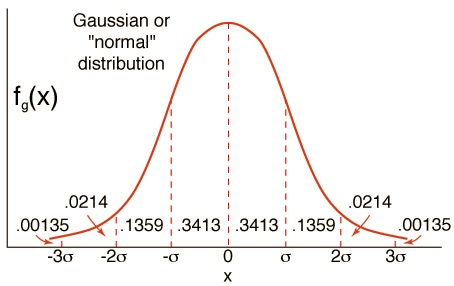
\includegraphics[scale = 0.7]{gaussian}
\begin{equation}
    \sigma = \sqrt{N*M*(1-p)}
\end{equation}
Expressão para a determinar o valor do Trigger:
\begin{equation}
    Trigger = E + K*\sigma
\end{equation}
, em que K é o "nível de trigger", ou seja, a variável com a qual escolhemos o grau de complexidade desejado para as configurações.
\section{Eliminar falsos positivos}
\paragraph{}Apesar da fiabilidade do método descrito anteriormente, acrescentamos um passo para eliminar falsos positivos. Sendo o trigger acionado, corremos a função iterate sem probabilidade quântica. Se, após esta iteração, ainda houver células vivas, confirmamos que havia estruturas além do "ruído".
\paragraph{}O método agora descrito acaba por ser uma representação mais próxima da nossa ideia de vida. No entanto, limitámo-nos a usá-lo apenas para confirmação por várias razões: não é eficiente em termos computacionais; não permite, entre as estruturas complexas, avaliar quantitativamente a sua complexidade; interfere na própria simulação, por estar sucessivamente a "limpar o ruído".
\newpage
\section{Análise de Resultados}
\paragraph{} 
Utilizando o programa "Dev", corremos, para probabilidades desde 0.001 até a 0.01, iterações até ser acionado e trigger, cujo nível era 5 no primeiro gráfico e 10 no segundo gráfico. Através de uma análise superficial, é obvio que o número de iterações necessário para o surgimento de complexidade é menor quanto maior for a probabilidade quântica p.
\newline 
Por outro lado, comparando os resultados obtidos para os diferentes níveis de trigger, conclui-se que estes são muito semelhantes, sendo que o nível de trigger mais alto levou a um ligeiro aumento do tempo necessário para atingir a complexidade. Isto pode ser explicado pelo facto de as estruturas serem construídas de forma cumulativa (a partir do momento em que surge uma estrutura que consegue sobreviver, o aumento da complexidade é mais rápido que o verificado anteriormente), com estruturas muito complexas a serem formadas a partir de modificações de estruturas mais simples.
\begin{center}
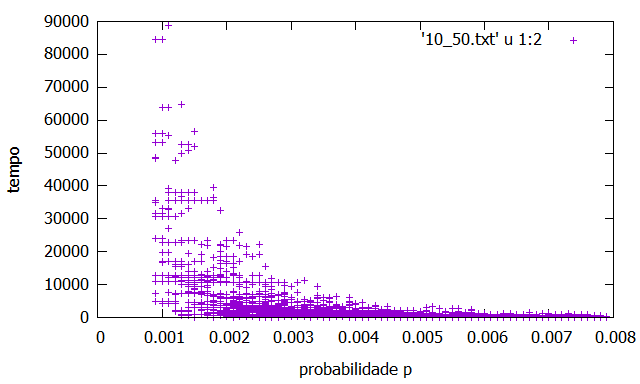
\includegraphics[scale=0.5]{plot_trigger_10.png}
\newline
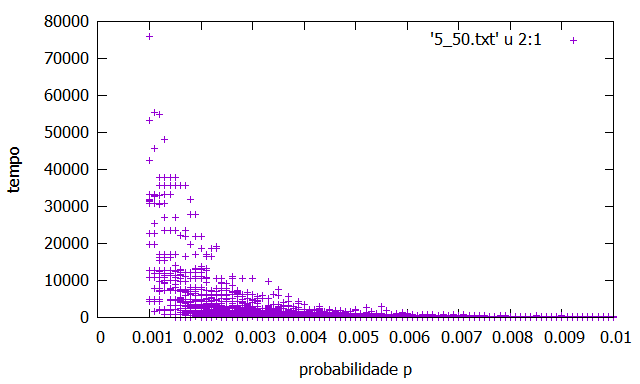
\includegraphics[scale=0.5]{plot_trigger_5.png}
\end{center}

\section{Algumas configurações espontâneas}
\subsection{Trigger level 5}

\fbox{
\includegraphics[width = 10 cm,height = 10 cm]{Trigger_5/1}}
\newline
\fbox{
\includegraphics[width = 10 cm,height = 10 cm]{Trigger_5/2}}
\newline
\fbox{
\includegraphics[width = 10 cm,height = 10 cm]{Trigger_5/3}}
\newline
\fbox{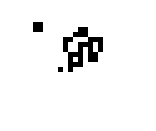
\includegraphics[width = 10 cm,height = 10 cm]{Trigger_5/4}}
\newline
\fbox{
\includegraphics[width = 10 cm,height = 10 cm]{Trigger_5/5}}
\newline

\subsection{Trigger level 10}
\fbox{
\includegraphics[width = 10 cm,height = 10 cm]{Trigger_10/1}}
\newline
\fbox{
\includegraphics[width = 10 cm,height = 10 cm]{Trigger_10/2}}
\newline
\fbox{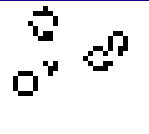
\includegraphics[width = 10 cm,height = 10 cm]{Trigger_10/3}}
\newline
\fbox{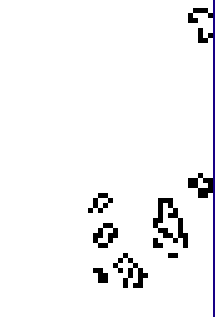
\includegraphics[width = 10 cm,height = 10 cm]{Trigger_10/4}}
\newline
\fbox{
\includegraphics[width = 10 cm,height = 10 cm]{Trigger_10/5}}
\newline

\end{document}
